\documentclass[a3paper,12pt]{extarticle} % Use extarticle for A3 paper size
\usepackage{graphicx} % Include this package for \includegraphics
\usepackage{amsmath}
\usepackage{amssymb} % Include this package for \mathbb
\usepackage[margin=1in]{geometry} % Adjust the margin as needed

\begin{document}

\author{kipngeno koech - bkoech}
\title{Homework 3 - Introduction to Machine Learning for Engineers}   
\maketitle

\medskip

\maketitle
\section{Dimensionality of K-Nearest Neighbors}

When the number of features $d$ is large, the performance of $k$-nearest neighbors, which makes predictions using only observations that are near the test observation, tends to degrade. This phenomenon is known as the \textit{curse of dimensionality}, and it ties into the fact that non-parametric approaches often perform poorly when $d$ is large.

\begin{enumerate}
    \item Suppose that we have a set of training observations, each corresponding to a one-dimensional ($d = 1$) feature, $X$. We assume that $X$ is uniformly (evenly) distributed on $[0, 1]$. Associated with each training observation is a response value.Suppose that we wish to predict a test observation $x$'s response using only training observations that are within $10\%$ of the range of $x$ closest to that test observation. In other words, if $x \in [0.05, 0.95]$ then we will use training observations in the range $[x - 0.05, x + 0.05]$, as shown in Figure 1 when $x = 0.6$. When $x \in [0, 0.05)$ we use the range $[0, 0.1]$, and when $x \in (0.95, 1]$ we use training observations in the range $[0.9, 1]$. Figure 1 shows this range for $x = 0.02$.On average (assuming $x$ is uniformly distributed on $[0, 1]$), what fraction of the available observations will we use to make the prediction?
    \item Now suppose that we have a set of observations, each corresponding to two features, $X_1$ and $X_2$ (i.e., $d = 2$). We assume that $(X_1, X_2)$ are uniformly distributed on $[0, 1] \times [0, 1]$. We wish to predict the response of a test observation $(x_1, x_2)$ using only training observations that are within $10\%$ of the range of $x_1$ and within $10\%$ of the range of $x_2$ closest to that test observation. For instance, in order to predict the response for a test observation with $x_1 = 0.6$ and $x_2 = 0.04$, we will use training observations $(X_1, X_2)$ such that $X_1 \in [0.55, 0.65]$ and $X_2 \in [0, 0.1]$.
    \begin{figure}[h]
        \centering
        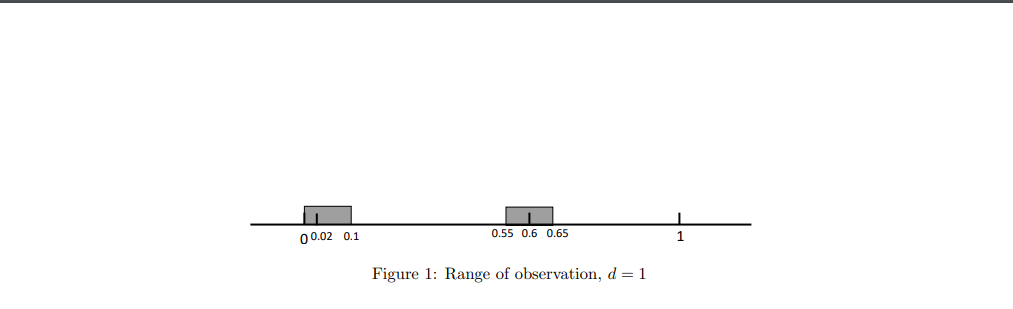
\includegraphics[width=0.8\textwidth]{section1.png}
        \caption{Primal Formulation of SVM}
        \label{fig:primal}
    \end{figure}
    \item On average, assuming $x_1$ and $x_2$ are each uniformly distributed on $[0, 1]$, what fraction of the available observations will we use to make the prediction?
    \item Now suppose that we have a set of training observations on $d = 100$ features. Again, the observations are uniformly distributed on each feature, and again each feature ranges in value from $0$ to $1$. We wish to predict a test observation’s response using observations within the $10\%$ of each feature’s range that is closest to that test observation. What fraction of the available observations will we use to make the prediction?
    \item Using your answers to parts a–c, argue that a drawback of $k$-nearest neighbors when $d$ is large is that there are very few training observations “near” any given test observation.
    \item Now suppose that we wish to make a prediction for a test observation by creating a $d$-dimensional hypercube centered around the test observation that contains, on average, $10\%$ of the training observations. For $d = 1$, $2$, and $100$, what is the length of each side of the hypercube? How does your answer change as $d$ increases, and what does this imply for the accuracy of $k$-nearest neighbors when $d$ is large?
    
    \textbf{Note:} A hypercube is a generalization of a cube to an arbitrary number of dimensions. When $d = 1$, a hypercube is simply a line segment; when $d = 2$, it is a square; and when $d = 100$, it is a $100$-dimensional cube.
\end{enumerate}
\newpage

\section{Decision Trees}
You obtained the following data from interviewing 15 people on the street. Based on a person’s relationship
status, age, education level and income, you can now build a decision tree to predict a person’s phone usage.
\begin{figure}[h]
    \centering
    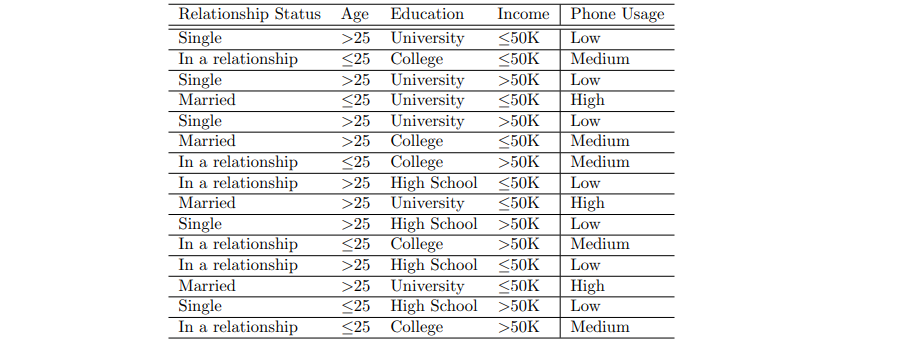
\includegraphics[width=0.8\textwidth]{section2.png}
    \caption{Primal Formulation of SVM}
    \label{fig:primal}
\end{figure}

\begin{enumerate}
    \item What is the entropy of Phone Usage? (Calculate entropy in log2 base and round to 4 decimal places)
    \item Find the information gain (IG) from each feature (relationship status, age, education levarianceel and income). Which feature should be chosen at the root of the tree? Show your calculations for the information gain (IG) and explain your choice in a sentence. (Calculate entropy in log2 base and round to 4 decimal places)
    \item  Use the root you found in part (b) to determine the rest of the nodes in the decision tree for the abovariancee data. Draw the full decision tree, i.e., keep splitting the nodes until further splits do not lead to any information gain (you may not need all the features for this). For each split, show your working on why you chose this feature based on information gain.
\end{enumerate}
\newpage
\section{Random Forests}
Consider the data samples in Table 1, which record whether a person gets sick, together with features about their age ($A$), social distancing ($S$), and hand-washing frequency ($H$). Our goal is to learn a random forest to predict whether the person is prone to getting sick.
\begin{table}[h!]
    \centering
    \begin{tabular}{|c|c|c|c|c|}
    \hline
    \textbf{Sample} & \textbf{Age (A)} & \textbf{Social Distancing (S)} & \textbf{Hand Washing (H)} & \textbf{Getting Sick} \\ \hline
    1 & Old & Yes & Yes & No \\ \hline
    2 & Old & Yes & No & No \\ \hline
    3 & Old & Yes & Yes & No \\ \hline
    4 & Young & No & No & Yes \\ \hline
    5 & Young & Yes & Yes & No \\ \hline
    6 & Old & No & No & Yes \\ \hline
    7 & Old & No & Yes & Yes \\ \hline
    8 & Old & No & No & Yes \\ \hline
    \end{tabular}
    \caption{}
    \label{table:data}
    \end{table}

    Instead of using all features to build a single decision tree, we decide to use the random forest algorithm. Specifically, we will build three trees, each using only two features, and then combine their outcomes for the final prediction.

    \begin{enumerate}
        \item  Build 3 decision trees using two features out of the three for each tree. Use information gain to decide the feature to split on. Use majority voting if all the samples in a leaf node do not have the same label.
        \item  Given a new data point with the features ($A = \text{old}$, $S = \text{yes}$, $H = \text{no}$), use the trees you learned from part (a) to predict whether this person will get sick.
        \item  Briefly (in 1-2 sentences) comment on the advantage of random forests over decision trees from the perspective of bias-variance trade-off.
    \end{enumerate}

\newpage
\section{Adaboost}
Recall the AdaBoost algorithm for classification of a training dataset $(x_n, y_n)$ for $n = 1, \dots, N$ and $y \in \{-1, 1\}$. AdaBoost sequentially combines $T$ weak classifiers $h_1(x), h_2(x), \dots, h_T(x)$ to build one strong classifier $\text{sign}(f_T(x))$. The steps of the algorithm are as follows:

\begin{itemize}
    \item \textbf{Initialize the weights:} $w_1(n) = \frac{1}{N}$, for all points $n = 1, 2, \dots, N$.
    \item \textbf{For $t = 1, \dots, T$:}
    \begin{itemize}
        \item \textbf{a.} Learn classifier $h_t(x)$ that minimizes the error:
        \[
        \epsilon_t = \sum_{n=1}^N w_t(n) \cdot \mathbb{1}(y_n \neq h_t(x_n)).
        \]
        \item \textbf{b.} Update the contribution:
        \[
        \beta_t = \frac{1}{2} \log_2\left(\frac{1 - \epsilon_t}{\epsilon_t}\right).
        \]
        \item \textbf{c.} Update weights of training points:
        \[
        w_{t+1}(n) \propto w_t(n) \cdot 2^{-\beta_t y_n h_t(x_n)},
        \]
        where the weights are normalized to ensure that $\sum_{n=1}^N w_{t+1}(n) = 1$.
    \end{itemize}
    \item \textbf{Return the final classifier:} $\text{sign}(f_T(x))$, where
    \[
    f_T(x) = \sum_{t=1}^T \beta_t h_t(x) \quad \text{for a given } x.
    \]
\end{itemize}

\textbf{Note:} The difference from the algorithm described during the lecture is that we have replaced $\log_e$ by $\log_2$ and $e^{-\beta_t}$ by $2^{-\beta_t}$ everywhere.
\begin{figure}[h]
    \centering
    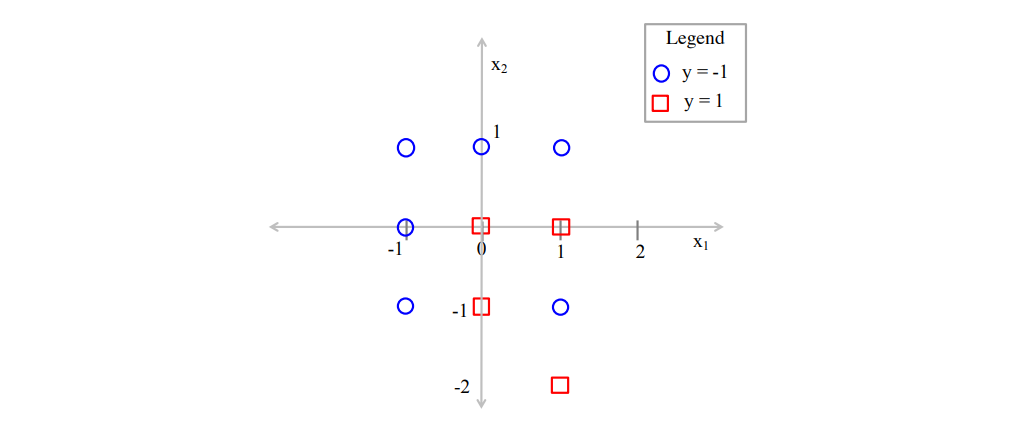
\includegraphics[width=0.8\textwidth]{adaboost.png}
    \caption{Primal Formulation of SVM}
    \label{fig:primal}
\end{figure}

Consider the training dataset with $N = 10$ points and two-dimensional features $x = (x_1, x_2)$ as shown in the figure above. In this problem, we will use a binary linear decision boundary as the base classifier and perform two iterations of AdaBoost.

\begin{enumerate}
    \item  Starting with equal weights $w_1(n) = \frac{1}{10}$ for all $N = 10$ points, which of the decision boundaries shown below gives the lowest error $\epsilon_1$? Select one of the following answers:

\begin{enumerate}
    \item Predict $y = 1$ if $x_2 \leq 0.5$.
    \item  Predict $y = 1$ if $-x_1 + x_2 \leq -0.5$.
    \item  Predict $y = 1$ if $-x_1 + x_2 \leq 0.5$.
\end{enumerate}

\begin{figure}[h!]
    \centering
    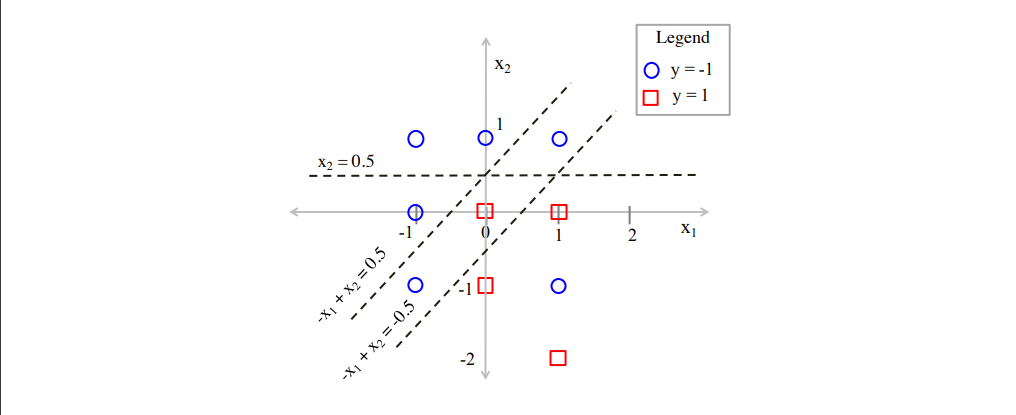
\includegraphics[width=0.8\textwidth]{adaboost2.png}
    \caption{Primal Formulation of SVM}
    \label{fig:primal}
\end{figure}


    \item Compute the error $\epsilon_1$ and the contribution $\beta_1$ of the decision boundary that you chose in part (a) above.

\item  Compute the updated and normalized weights $w_2(n)$ of each of the data points as follows:

\begin{table}[h!]
\centering
\begin{tabular}{|c|c|c|}
\hline
\textbf{n} & \textbf{Coordinates} & \textbf{$w_2(n)$} \\ \hline
1. & $(-1, 1)$ & \\ \hline
2. & $(0, 1)$ & \\ \hline
3. & $(1, 1)$ & \\ \hline
4. & $(-1, 0)$ & \\ \hline
5. & $(0, 0)$ & \\ \hline
6. & $(1, 0)$ & \\ \hline
7. & $(-1, -1)$ & \\ \hline
8. & $(0, -1)$ & \\ \hline
9. & $(1, -1)$ & \\ \hline
10. & $(1, -2)$ & \\ \hline
\end{tabular}
\caption{}
\label{table:weights}
\end{table}

\item Suppose you are given one more weak classifier that predicts $y = 1$ if $1.5x_1 + x_2 \leq 0.5$, as shown in the figure below. Compute the contribution $\beta_2$ of this classifier for the updated set of weights $w_2(n)$. Use the approximation $\log_2 3 \approx 1.6$.

\item Combine the new classifier with the classifier that you obtained in part (a). Specify the label $y \in \{-1, 1\}$ predicted by this combined classifier for each data point. Do you observe any change in the prediction, compared to the prediction from only using part (a)'s classifier?

\item  If we continue adding more classifiers, each with error less than $0.5$, how does the training error of the combined classifier $f_T(x)$ change? Briefly explain your answer in 1-2 sentences.

\newpage
\section{Neural Networks}
\end{enumerate}










\end{document}